\documentclass[12pt,answers]{exam}
\usepackage[margin=0.5in]{geometry}
\usepackage{amsmath,amssymb}
\usepackage{tikz}
\usetikzlibrary{arrows,automata,positioning}
\usepackage{soul}

\newcommand{\blank}[1]{\underline{\hspace*{#1}}}
\newcommand{\ds}{\displaystyle}
\newcommand{\on}{\operatorname}
\newcommand{\mymod}{~\mathrm{mod}~}


\begin{document}
\pagestyle{empty}
\graphicspath{{/home/brian/Dropbox/HSC/Spring16/Math111/}}

\subsubsection*{COMS 461 - Midterm 1 Review Solutions}

\begin{questions}

\question[8] Consider the DFA shown below. 
\begin{center}
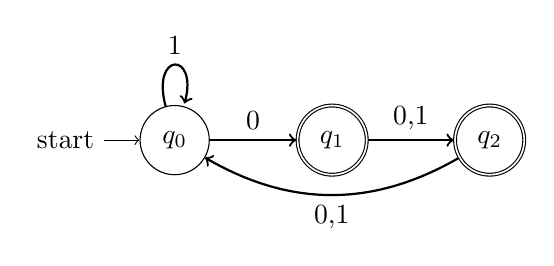
\begin{tikzpicture}[node distance=2cm,auto]
  \node[state,initial]   (q_0)                 {$q_0$};
  \node[state,accepting] (q_1) [right of=q_0]  {$q_1$};
  \node[state,accepting] (q_2) [right of=q_1]  {$q_2$};
  \path[thick,->]
  (q_0) edge              node {0} (q_1)
        edge [loop above] node {1} ()
  (q_1) edge              node {0,1} (q_2)
  (q_2) edge [bend left] node {0,1} (q_0);
\end{tikzpicture}
\end{center}

\begin{parts}
\part What sequence of states will this DFA enter as it reads the string 110101?
\begin{solution}
$$q_0 \rightarrow q_0 \rightarrow q_0 \rightarrow q_1 \rightarrow q_2 \rightarrow q_0 \rightarrow q_0$$
\end{solution}
\vfill

\part Will this DFA accept the string 110101?
\begin{solution}
No, it will not accept that string because it ends in state $q_0$. 
\end{solution}
\vfill
\end{parts}

\question[16] The following statements are all false.  For each one, explain why it is false.  
\begin{parts}
\part The cardinality of $\{0,1\}^*$ is uncountable.
\begin{solution}
This is false because $\{0,1\}^*$ is countably infinite. It is a countable union of finite sets. % You can put the strings in lexicographic ordering and then count them.
\end{solution}
\vfill


\part The $\on{NAND}$ function is universal which means that any function $f:\{0,1\}^* \rightarrow \{0,1\}$ can be expressed using $\on{NAND}$ functions. 
\begin{solution}
This is false because NAND can only compute all Boolean valued functions defined on binary strings of a fixed finite length, not arbitrary length.  Universal means that all function $f:\{0,1\}^n \rightarrow \{0,1\}$ can be expressed using $\on{NAND}$ functions for any fixed $n$.
\end{solution}
\vfill

\part The union of any two languages $A, B \subset \{0,1\}^*$ is a regular language.  
\begin{solution}
This is false unless you also assume that $A$ and $B$ are both regular languages.
\end{solution}
\vfill

%\part All finite languages are regular and have a pumping number of 1.  
%\vfill

\part Boolean logic circuits, DFAs, NFAs, and regular expressions are all equivalent computationally.  They are all able to recognize regular languages.
\begin{solution}
Every regular language can be checked with an NFA or DFA or expressed with a regular expression, but not every regular language can be checked by a Boolean logic circuit.
\end{solution}
\vfill

\end{parts}


%\question Let $f: \{0,1\}^4 \rightarrow \{0,1\}$ be defined by $(x_0 \wedge x_1) \vee (x_2 \wedge x_3)$. 
%\begin{parts}
%\part What is $f(0,0,1,1)$?  
%\begin{solution}
%$f(0,0,1,1) = 1$
%\end{solution}
%\vfill
%
%\part Find a different formula for $f(x_0,x_1,x_2,x_3)$ using only $\on{NAND}$ functions.  
%\begin{solution}
%$\on{NAND}(\on{NAND}(x_0,x_1),\on{NAND}(x_2,x_3))$
%\end{solution}
%\end{parts} 
%\vfill
%\question Find a DFA that accepts a string $x \in \{0,1\}^*$ if and only the first three symbols in $x$ satisfy $\on{NAND}(\on{NAND}(x_0,x_1),x_2) = 1$.  

\newpage

\question[12] Let $L \subset \{0,1\}^*$ be the language that contains all strings with at least one 1 and at most one 0.  Construct a DFA that accepts $L$.  
\begin{solution}
\begin{center}
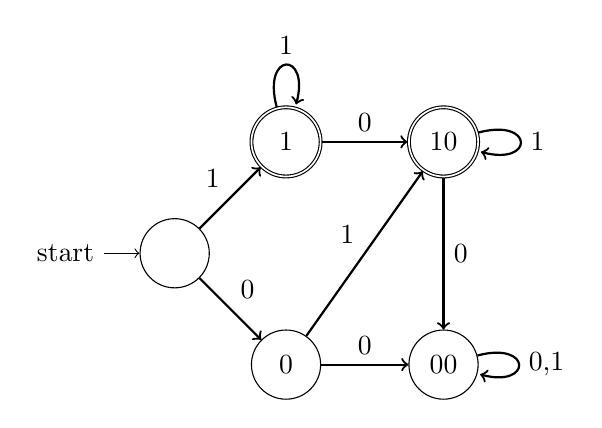
\begin{tikzpicture}[node distance=2cm,auto]
  \node[state,initial]   (qb)                 {$ $};
  \node[state,accepting] (q_1) [above right of=qb] {$1$};
  \node[state,accepting] (q_10) [right of=q_1] {$10$};
  \node[state]           (q_0) [below right of=qb] {$0$};
  \node[state]           (q_00) [right of=q_0]  {$00$};
  \path[thick,->]
  (qb) edge              node {1} (q_1)
  (qb) edge              node {0} (q_0)
  (q_0) edge             node {1} (q_10)
  (q_0) edge             node {0} (q_00)
  (q_1) edge[loop above] node {1} ()
  (q_1) edge             node {0} (q_10)
  (q_00) edge[loop right] node {0,1} ()
  (q_10) edge[loop right] node {1} ()
  (q_10) edge             node {0} (q_00);
\end{tikzpicture}
\end{center}
\end{solution}
\vfill
\vfill


\question[16] Consider the regular expression $(00)^*1(0|1)$.
\begin{parts}

\part Describe in words the set of strings that this regular expression will match. 
\begin{solution}
Any string that combines an even number of zeros with either a 10 or 11 at the end.  
\end{solution}
\vfill

\part Construct an NFA (or DFA) that accepts exactly that set of strings. 
\begin{solution}
\begin{center}
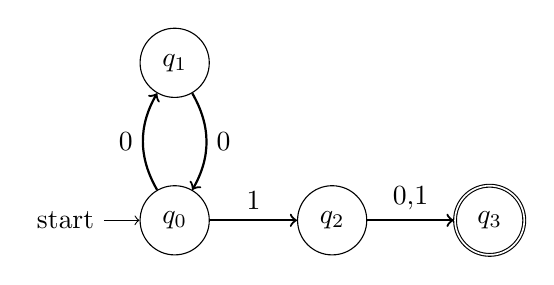
\begin{tikzpicture}[node distance=2cm,auto]
  \node[state,initial]   (q_0)                 {$q_0$};
  \node[state]           (q_1) [above of=q_0] {$q_1$};
  \node[state]           (q_2) [right of=q_0] {$q_2$};
  \node[state,accepting] (q_3) [right of=q_2] {$q_3$};
  \path[thick,->]
  (q_0) edge[bend left] node {0} (q_1)
  (q_1) edge[bend left] node {0} (q_0)
  (q_0) edge             node {1} (q_2)
  (q_2) edge             node {0,1} (q_3);
\end{tikzpicture}
\end{center}
\end{solution}

\vfill
\vfill

\end{parts}


\newpage
\question[8] In biology, strings of three DNA nucleotides (called \emph{codons}) are known to encode 20 different amino acids.  Here, the alphabet consists of the four DNA nucleotides $\Sigma = \{A, C, G, T\}$. Let $\mathcal{A}$ denote the set of 20 possible amino acids.
\begin{parts}
\part How many possible strings of three nucleotides are there? In other words, find $|\Sigma^3|$.
\begin{solution}
There are $4^3 = 64$ possible strings of length three from $\{A,C,G,T\}$.
\end{solution}
\vfill

\part How many possible functions are there from $\Sigma^3 \rightarrow \mathcal{A}$?
\begin{solution}
There are $20^{64}$ possible functions from $\Sigma^3$ to $\mathcal{A}$.
\end{solution}
\vfill
\end{parts}

\question[8] Consider the DFA shown below.

\begin{center}
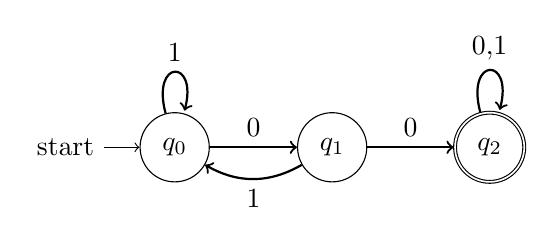
\begin{tikzpicture}[node distance=2cm,auto]
  \node[state,initial]   (q_0)                 {$q_0$};
  \node[state]           (q_1) [right of=q_0]  {$q_1$};
  \node[state,accepting]           (q_2) [right of=q_1]  {$q_2$};
  \path[thick,->]
  (q_0) edge              node {0} (q_1)
        edge [loop above] node {1} ()
  (q_1) edge              node {0} (q_2)
  (q_1) edge [bend left]  node {1} (q_0)
  (q_2) edge [loop above] node {0,1} ();
\end{tikzpicture}
\end{center}

\begin{parts}
\part This DFA can be described by a quintuple $(Q,\Sigma,\delta,q,F)$ where $\Sigma = \{0,1\}$.  What are $Q$, $q$ and $F$ in this notation?  
\begin{solution}
$Q = \{q_0, q_1, q_2 \}$, $q = q_0$, and $F = \{q_2\}$. 
\end{solution}
\vfill


\part Find a regular expression that matches the same set of strings that this DFA accepts.  
\begin{solution}
$$(0|1)^*00(0|1)^*$$
\end{solution}
\vfill


\end{parts}







\newpage
%\question Prove or disprove the following claim: There is a regular expression that can recognize the language $L \subset \{0,1\}^*$ consisting of all strings with more 0's than 1's.  
\question[12] Let $L \subset \{0,1\}^*$ be the language consisting of all strings with more 0's than 1's. Use the pumping lemma to prove that $L$ is not regular.  
\begin{solution}
If $L$ is regular, then it has a pumping number $p$.  Consider the string $1^p 0^{p+1}$.  If you pump this string, then you will increase the number of 1's, which will give you a string not in $L$.  That is a contradiction, so $L$ is not regular.
\end{solution}
\vfill


\question[20] Let $\Sigma = \{0, 1, +, =\}$ and let 
$$L = \{x=y+z : x, y, z \text{ are binary integers, and }x\text{ is the sum of }y\text{ and }z\}.$$
\begin{parts}
\part Which of the following strings are in $L$?  Circle all correct answers, there might be more than one.
\begin{choices}
\choice \verb|100=1+10|
\CorrectChoice \verb|11=10+1|
\choice \verb|2=1+1|
\CorrectChoice \verb|1000=111+1|
\choice \verb|x=11+z, if y=11|
\end{choices}
\bigskip


%\part Give an example of a string in $L$. 
%\begin{solution}
%\begin{center}
%\verb|11=10+1|
%\end{center}
%\end{solution}
%\vfill

\part Is it possible to write a regular expression over $\Sigma$ that represents all valid strings in $L$? Explain why or why not. 
\begin{solution}
No, there is no regular expression for this language because it is not regular.  If it were regular, there would be a pumping length $p$, such that any string longer than $p$ in $L$ could be pumped. But a string that begins with $p$ 1's could not be pumped since adding more ones to the binary number on the left side of the equality will make the equation not true.
\end{solution}
\vfill

\end{parts}

\end{questions}

\end{document}
